\documentclass[compress]{beamer}

\usetheme{Hamburg}

\usepackage[T1]{fontenc}
\usepackage[utf8]{inputenc}

\usepackage{lmodern}

\usepackage[english]{babel}
%\usepackage[ngerman]{babel}

\usepackage{eurosym}
\usepackage{listings}
\usepackage{microtype}
\usepackage{units}
\usepackage{hyperref}
\usepackage{url}


\lstset{
	basicstyle=\ttfamily\footnotesize,
	frame=single,
	numbers=left,
	language=C,
	breaklines=true,
	breakatwhitespace=true,
	postbreak=\hbox{$\hookrightarrow$ },
	showstringspaces=false,
	tabsize=4,
	captionpos=b,
	morekeywords={gboolean,gpointer,gconstpointer,gchar,guchar,gint,guint,gshort,gushort,glong,gulong,gint8,guint8,gint16,guint16,gint32,guint32,gint64,guint64,gfloat,gdouble,gsize,gssize,goffset,gintptr,guintptr,int8_t,uint8_t,int16_t,uint16_t,int32_t,uint32_t,int64_t,uint64_t,size_t,ssize_t,off_t,intptr_t,uintptr_t,mode_t}
}

\title{I/O analysis of climate applications}
\author{Arne Beer \& Frank Röder}
\institute{Arbeitsbereich Wissenschaftliches Rechnen\\Fachbereich Informatik\\Fakultät für Mathematik, Informatik und Naturwissenschaften\\Universität Hamburg}
\date{2016-07-7}

\titlegraphic{
\includegraphics[width=0.75\textwidth]{gfx/logo}}

\begin{document}

\begin{frame}
	\titlepage
\end{frame}

\begin{frame}
	\frametitle{Content (Agenda)}

	\tableofcontents[hidesubsections]
\end{frame}

\section{Introduction}
\begin{frame}
	\frametitle{Introduction}

    \begin{itemize}
		\item Why we use models
		\begin{itemize}
			\item simulations
			\item another part of nowadays research
		\end{itemize}
	\end{itemize}

	\begin{itemize}
		\item Climate applications
		\begin{itemize}
			\item about the I/O
			\item analysis
			\item different Models
			\item visualisation
		\end{itemize}
	\end{itemize}
\end{frame}

\begin{frame}
    \frametitle{Motivation}
    \begin{itemize}
		\item models need huge amounts of data
        \item data storage is limited and expensive
        \item analyse models and evaluate needed data
        \item prune as much data as possible
	\end{itemize}
\end{frame}

\section{Models}
\begin{frame}
    \frametitle{What are models}

    \begin{itemize}
		\item Climate Models
		\begin{itemize}
			\item a representation of climate
			\item ocean, ice, land, river, vegetation
			\item predict future climate
			\item global scale
		\end{itemize}
		\item Atmospherical model
		\begin{itemize}
			\item numerical weather prediction
			\item predict weather in a foreseeable period
		\end{itemize}
    \end{itemize}

\end{frame}


\subsection{Input and Output}

\begin{frame}[fragile]
	\frametitle{Structure of the data}

		\begin{itemize}
		    \item numeric data
			\item scalar quantities
			\item vectors
			\item grid data
		\end{itemize}

\end{frame}

\subsection{File Format}

\begin{frame}[fragile]
	\frametitle{Most important formats used for climate applications}

		\begin{itemize}
			\item netCDF
			\item HDF5
			\item since version 4 netCDF is embedded in HDF5
		\end{itemize}

  \begin{figure}[htbp]
    \begin{minipage}{0.35\textwidth}
     \centering
      
\includegraphics[width=0.8\textwidth]{gfx/hdf.jpg}
      \caption{hdf-logo \cite{hdf}}
    \end{minipage}\hfill
    \begin{minipage}{0.35\textwidth}
     \centering
      
\includegraphics[width=0.8\textwidth]{gfx/netcdf.png}
      \caption{netcdf-logo \cite{netcdf}}
    \end{minipage}
  \end{figure}

\end{frame}


\subsection{The model landscape}

\begin{frame}
    \frametitle{The model landscape}
	\begin{itemize}
		\item large choice
		\item old models
		\item poorly documented
		\item nearly no open source
		\item example IFS
	\end{itemize}

\end{frame}

\section{Awips II}
\begin{frame}
    \frametitle{Awips II}
    \begin{center}
    	\begin{figure}
			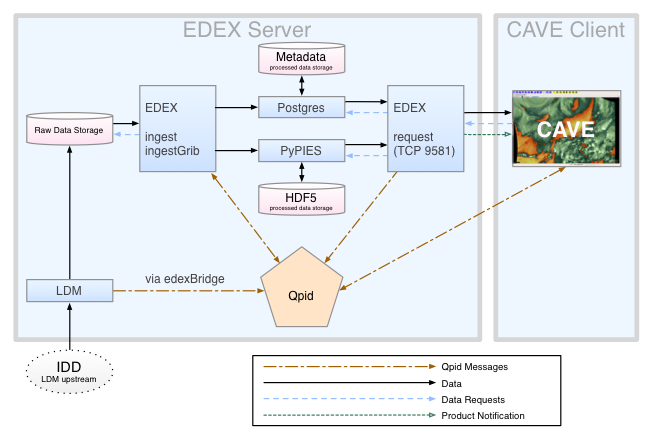
\includegraphics[width=0.7\textwidth]{gfx/awipsII.png}
      	  	\caption[]{Awips Infrastructure \cite{Uni01}}
		\end{figure}
	\end{center}

\end{frame}

\begin{frame}
    \frametitle{Awips II}
    	\begin{itemize}
			\item forecast display and analysis
			\item provides EDEX to store computed data \cite {AwipsDocs}
	    	\begin{itemize}
		    	\item HDF5 Storage
		    	\item custom python libraries for storage management
		    	\item PostgreSQL for metadata management and storage
		    \end{itemize}
		    \item Provides CAVE to display data
	    	\begin{itemize}
		    	\item program to connect with EDEX server
		    	\item select data set, download and view it on your local machine
		    \end{itemize}
		\end{itemize}
\end{frame}

\section{CESM}
\begin{frame}
    \frametitle{CESM}
    	\begin{itemize}
    	    \item Community Earth System Model
			\item model for global climate simulation
			\item covers atmosphere, land, land ice, sea ice, ocean and river
			\item provides scripts for setting up the machine in 4 commands
	    	\begin{itemize}
		    	\item scripts are broken
		    	\item mix of bash, csh, perl
		    \end{itemize}
		    \item good configurability with xml files
		    \item requires netCDF format for input data \cite{CESMDocs}
		\end{itemize}
\end{frame}


\section{Summary}

\begin{frame}
	\frametitle{Summary}

	\begin{itemize}
		\item Data

		\begin{itemize}
			\item hdf5 , netCDF
		\end{itemize}

		\item Models
		\begin{itemize}
			\item CESM
			\item EcoHam
		\end{itemize}
		\item Analyzer
		\begin{itemize}
		    \item awips2
		\end{itemize}
	\end{itemize}
\end{frame}

\section*{Literature}

\begin{frame}[allowframebreaks]
	\frametitle{Literature}
    \frametitle{Sources}

	\bibliographystyle{alpha}
	\bibliography{literatur.bib}
\end{frame}

\end{document}
